%botanophobi2019haru-example.tex
% ABOUT: This is a very elementary example for the use of the beamer class
% inherited from upb2018.

\documentclass[
	% uncomment, if you want to print your presentation as a handout
	% with possibly more than one slide per a4page. You can choose
	% the number of slides printed on one handout-page below in the
	% options of \usetheme.
		%handout
	] {beamer}

\usepackage[T1]{fontenc}
\usepackage[utf8]{inputenc}
\usepackage[english]{babel}

\usetheme[
	% choose the color theme of the presentation 
		blue
		%red
		%green
	,
	% uncomment, if you want to use the optional short title instead
	% of the full title in the header. Note that the short title
	% is only displayed in one line.
		shortTitleInHeader
	,
		%oneslideonhandout			% one slide per page (landscape)
		%twoslidesonhandout 	% two slides per page
		fourslidesonhandout			% four slides per page (landscape) [default]
]{bp2019haru}


% IMAGES
% chooose the cropped background image on the titlepage
\renewcommand{\titleimage}{logo/Background.JPG}
\renewcommand{\headerlogo}{logo/ustclonglogo.png}
\renewcommand{\framelogo}{logo/ustcshortlogo.png}

% GENERAL INFORMATIONS
\title[Gene Co-expression Network]{基因共表达网络在水稻\\育种中应用}
\subtitle{AtGGM2014}
\institute{School of Life Science, USTC}
\author{Student T}
\date{Jan. 11st, 2019}

\begin{document}

% titlepage
\begin{frame}[plain]
	\titlepage
\end{frame}

\begin{frame}{General Settings 1}
	The beamer theme \colemph{upb2018} can be used with the command 
	\begin{center}
		\texttt{$\backslash$usetheme[<colortheme>]\{upb2018\}}
	\end{center}

	For the option \texttt{<colortheme>} you can choose out of
	\texttt{cyan}, \texttt{orange}, \texttt{green}, \texttt{cassis}, \texttt{blue} oder
	\texttt{red}.

	In addition you can use the option \texttt{shortTitleInHeader} to
	use the optional short title instead of the full title in the header. Note that
	the short title is only displayed in one line.
\end{frame}



\begin{frame}{General Settings 2}
	You can change the cropped image on the title page using

	\begin{center}
		\texttt{$\backslash$renewcommand\{$\backslash$titleimage\}\{<path>\}}.
	\end{center}

	Note that your image will be cropped automatically.

	\vfill

	In the same way you can change the logo which is used on the title page and
	in every header:
	\begin{center}
		\texttt{$\backslash$renewcommand\{$\backslash$headerlogo\}\{<path>\}}
	\end{center}
\end{frame}



\normalframetitle % from now on use the (default) normal frame title style
\begin{frame}{This is a frame title written in the usual way. It can also
be multiline.}
	For slides with a normal size of the frame title, you can use \texttt{$\backslash$normalframetitle}
	before \texttt{$\backslash$begin\{frame\}}. In this style, frame titles can
	also be multiline.

	This style is set by default.
\end{frame}



\smallframetitle % from now on use the small frame title style
\begin{frame}{This is a frame title written in the small, single-line way.}
	If you want to have a slide with a smaller title, use the command \texttt{$\backslash$smallframetitle} before \texttt{$\backslash$begin\{frame\}}. Note that in this
	style, frame titles are always single-line. A smaller frame title is useful if more space is needed on the slide.

	Lorem ipsum dolor sit amet, consectetur adipiscing elit, sed do eiusmod tempor
	incididunt ut labore et dolore magna aliqua. Ut enim ad minim veniam, quis
	nostrud exercitation ullamco laboris nisi ut aliquip ex ea commodo consequat.
	Lorem ipsum dolor sit amet, consectetur adipiscing elit, sed do eiusmod tempor 
	incididunt ut labore et dolore magna aliqua. Ut enim ad minim veniam, quis 
	nostrud exercitation ullamco. Lorem ipsum dolor sit amet, consectetur adipiscing
	elit, sed do eiusmod tempor  incididunt ut labore et dolore magna aliqua.
\end{frame}



\normalframetitle
\begin{frame}{Items}
	If you use  \texttt{$\backslash$colitem\ldots} instead of
	\texttt{$\backslash$item\ldots} while you create an item list, the item text
	will be printed in the color theme of the presentation.

	\vfill
	\begin{columns}
		\begin{column}{.45\linewidth}
			Using \texttt{$\backslash$item \ldots}:
			\begin{itemize}
				\item Item 1
					\begin{itemize}
						\item Subitem 1
						\item Subitem 2
					\end{itemize}
				\item Item 2
				\item Item 3
			\end{itemize}
		\end{column}
		\begin{column}{.45\linewidth}
			Using \texttt{$\backslash$colitem \ldots } at the first level:
			\begin{itemize}
				\colitem Item 1
					\begin{itemize}
						\item Subitem 1
						\item Subitem 2
					\end{itemize}
				\colitem{Item 2}
				\colitem{Item 3}
			\end{itemize}
		\end{column}
	\end{columns}
\end{frame}



% \begin{frame}{Additional ways to emphasize your text}
% 	With the commands \texttt{$\backslash$colemph\{\ldots\}} and
% 	\texttt{$\backslash$important\{\ldots\}} you can emphasize parts of your text
% 	in the \colemph{color theme} oder in \important{ustcred}.
% \end{frame}



\begin{frame}{Mathematics}
	Mathematical formulas can be used as usual \colemph{inline}, like for example
	\(a^2+b^2 = c^2\) or in \colemph{display} mode:
	\[\sum\limits_{k=0}^\infty q^k = \frac{1}{1-q}, \quad \forall q \in ]0,1[.\]
\end{frame}





\smallframetitle
\begin{frame}{Picture and The End}
	Of course, it is also possible to use images in the presentation.

	\vfill

	\begin{columns}
		\begin{column}{.5\linewidth}
			\begin{figure}
				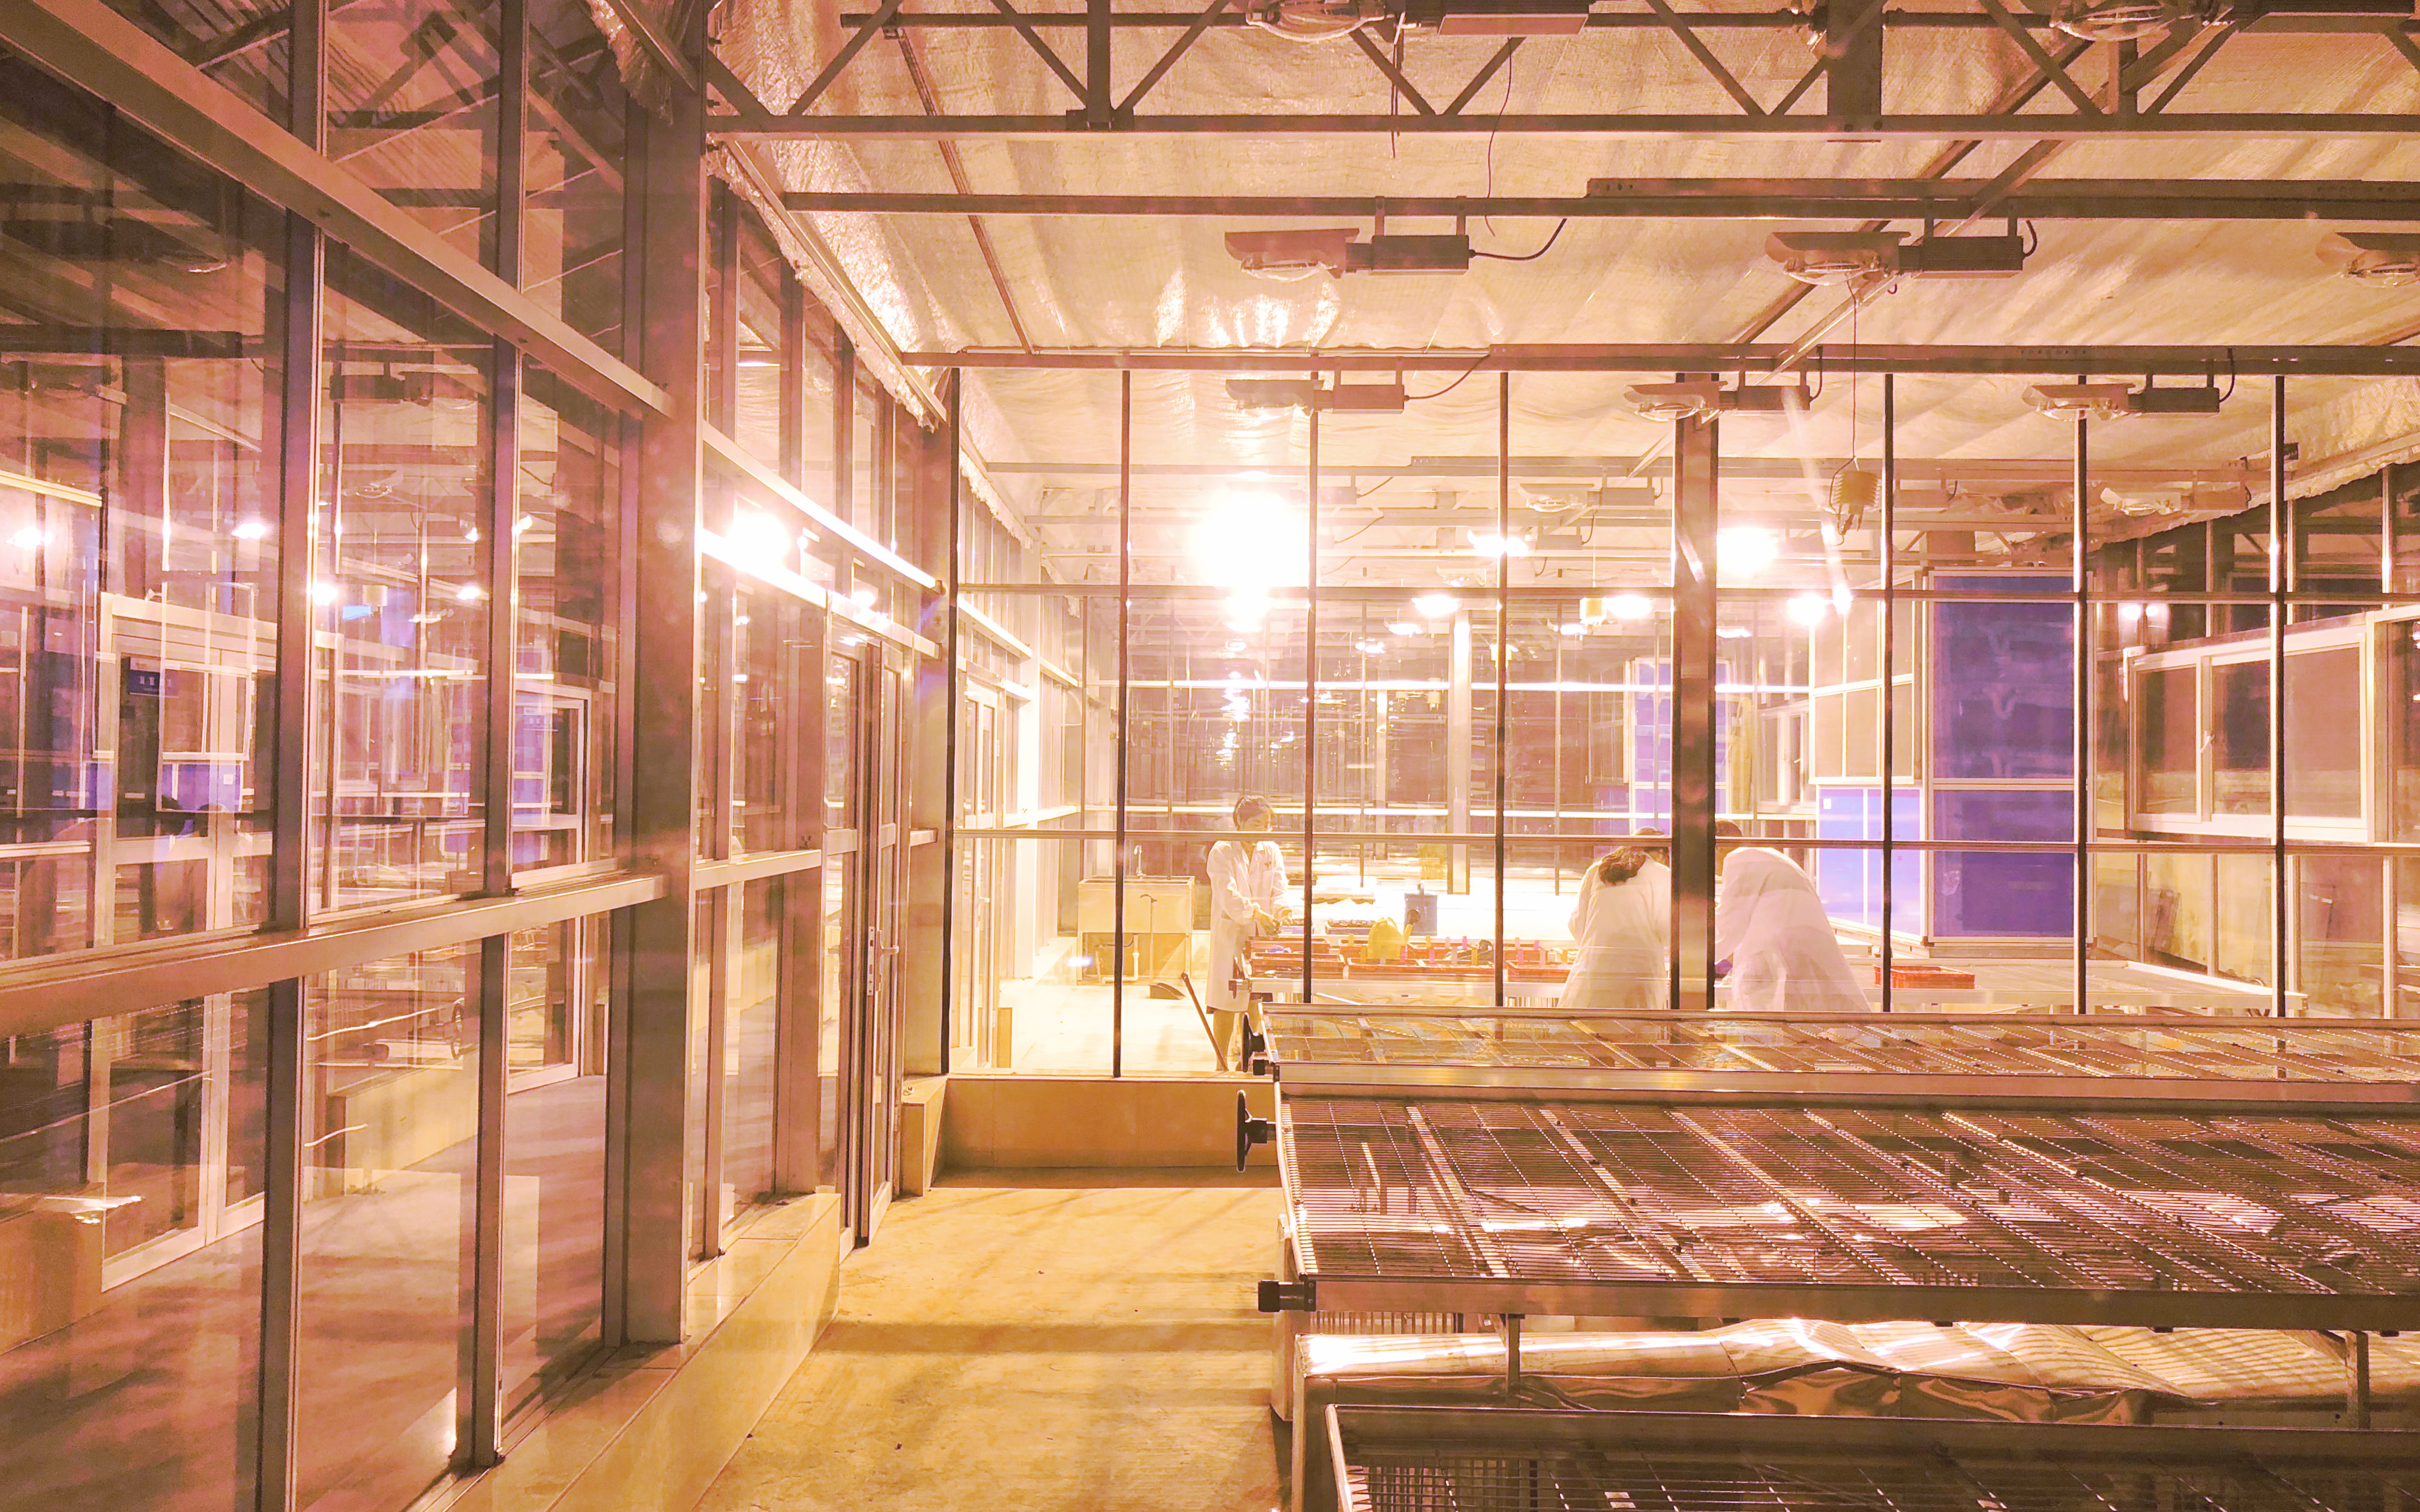
\includegraphics[width=.7\linewidth]{logo/Background.JPG}
				\caption{This is an imported image with a caption.}
				\label{abb:image}
			\end{figure}
		\end{column}
		\begin{column}{.5\linewidth}
			\LARGE \centering
			\colemph{Thank you} for your attention.
		\end{column}
	\end{columns}
\end{frame}



\end{document}
